\documentclass[border=4pt]{standalone}
\usepackage[utf8]{inputenc}
\usepackage{amsmath,amssymb}
\usepackage{tikz}
\usetikzlibrary{positioning,arrows.meta,calc,backgrounds,shapes.geometric}
\usepackage{xcolor}

% ── SD-inspired palette ──────────────────────────────────────
\definecolor{unetbg}{HTML}{E3EEDD}      \definecolor{unetbd}{HTML}{6FA85E}
\definecolor{condbg}{HTML}{F0F0F0}      \definecolor{condbd}{HTML}{9C9C9C}
\definecolor{rbBg}{HTML}{F8E6E1}        \definecolor{rbBd}{HTML}{C48378}
\definecolor{trapez}{HTML}{C9DEF3}      \definecolor{trapezB}{HTML}{3A6FB5}
\definecolor{resIcon}{HTML}{FDE2B6}     \definecolor{resIconB}{HTML}{C49045}
\definecolor{midIcon}{HTML}{D3E9CC}     \definecolor{midIconB}{HTML}{5E9844}
\definecolor{temb}{HTML}{FFEEBE}        \definecolor{tembB}{HTML}{B18E17}
\definecolor{skipc}{HTML}{8A8A8A}
\definecolor{concatBg}{HTML}{E8E0EF}    \definecolor{concatBd}{HTML}{8A6BB1}
\definecolor{samp}{HTML}{E6D3F0}        \definecolor{sampB}{HTML}{7A5BA0}

% Small wedge markers that physically convey spatial down-/up-sampling.
% Argument is a TikZ coordinate expression (e.g. (2,3) or ($(a)!0.5!(b)$)).
\newcommand{\downwedge}[1]{%
    \begin{scope}[shift={#1}]
        \filldraw[fill=samp, draw=sampB, line width=0.5pt]
            (-0.14, 0.22) -- (0.14, 0.10) --
            (0.14, -0.10) -- (-0.14, -0.22) -- cycle;
    \end{scope}%
}
\newcommand{\upwedge}[1]{%
    \begin{scope}[shift={#1}]
        \filldraw[fill=samp, draw=sampB, line width=0.5pt]
            (-0.14, 0.10) -- (0.14, 0.22) --
            (0.14, -0.22) -- (-0.14, -0.10) -- cycle;
    \end{scope}%
}

\begin{document}
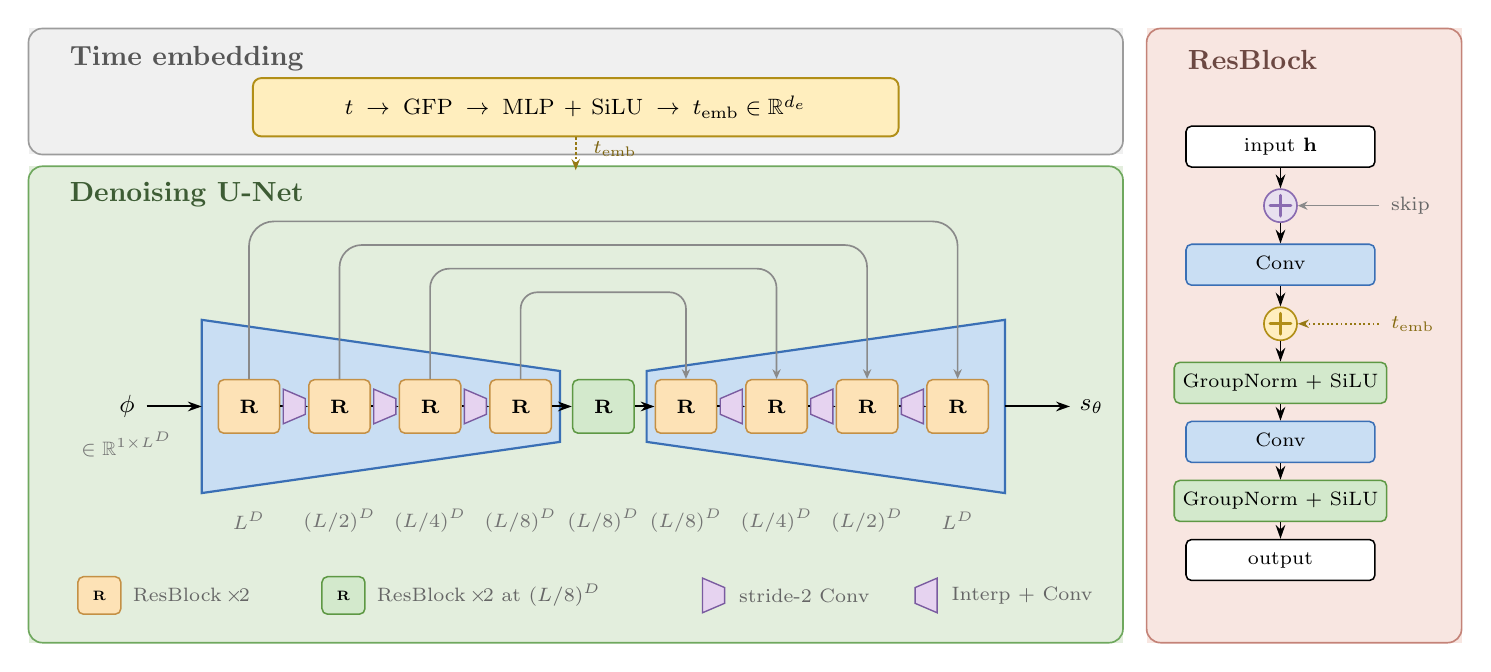
\begin{tikzpicture}[
    >=Stealth,
    ricon/.style={draw=resIconB, fill=resIcon, line width=0.55pt,
                  rounded corners=2pt,
                  minimum height=0.68cm, minimum width=0.78cm,
                  font=\scriptsize\bfseries, inner sep=1pt},
    micon/.style={draw=midIconB, fill=midIcon, line width=0.55pt,
                  rounded corners=2pt,
                  minimum height=0.68cm, minimum width=0.78cm,
                  font=\scriptsize\bfseries, inner sep=1pt},
    rb/.style={draw, line width=0.55pt, rounded corners=2pt, fill=white,
               minimum height=0.52cm, minimum width=2.40cm,
               align=center, font=\scriptsize, inner sep=3pt},
    rbconv/.style ={rb, fill=trapez,   draw=trapezB},
    rbnorm/.style ={rb, fill=midIcon,  draw=midIconB},
    % ⊕ circles — smaller, with the bold + drawn separately
    concatCirc/.style={circle, fill=concatBg, draw=concatBd,
                       line width=0.6pt, minimum size=0.42cm,
                       inner sep=0pt},
    tembCirc/.style  ={circle, fill=temb, draw=tembB,
                       line width=0.6pt, minimum size=0.42cm,
                       inner sep=0pt},
    arr/.style     ={-{Stealth[length=5pt,width=3.5pt]}, line width=0.7pt},
    sarr/.style    ={-{Stealth[length=3.5pt,width=3pt]}, line width=0.6pt,
                     color=skipc},
    % Down/up-sample markers: tiny trapezoid wedges whose shape
    % physically conveys spatial reduction / expansion.
    tarr/.style    ={densely dotted, tembB!85!black, line width=0.8pt,
                     -{Stealth[length=4pt,width=3pt]}},
    groupTitle/.style={font=\bfseries\normalsize, anchor=north west},
    reslbl/.style    ={font=\scriptsize, text=black!55},
    ioLbl/.style     ={font=\small},
]

% ═════════════════════════════════════════════════════════════
%  Section 1  ─  Time embedding (top strip)
% ═════════════════════════════════════════════════════════════
\begin{scope}[on background layer]
    \fill[condbg] (-0.40, 2.95) rectangle (13.50, 4.55);
    \draw[condbd, line width=0.6pt, rounded corners=5pt]
        (-0.40, 2.95) rectangle (13.50, 4.55);
\end{scope}

\node[groupTitle, text=condbd!55!black] at (0.00, 4.45)
    {Time embedding};

\node[fill=temb, draw=tembB, line width=0.7pt, rounded corners=3pt,
      minimum height=0.74cm, minimum width=8.2cm, font=\footnotesize]
    (temb) at (6.55, 3.55)
    {$t \;\to\; \text{GFP} \;\to\; \text{MLP}\,+\,\text{SiLU} \;\to\; t_{\mathrm{emb}}\in\mathbb{R}^{d_e}$};

% ═════════════════════════════════════════════════════════════
%  Section 2  ─  Denoising U-Net
% ═════════════════════════════════════════════════════════════
\begin{scope}[on background layer]
    \fill[unetbg] (-0.40, -3.25) rectangle (13.50, 2.80);
    \draw[unetbd, line width=0.6pt, rounded corners=5pt]
        (-0.40, -3.25) rectangle (13.50, 2.80);
\end{scope}

\node[groupTitle, text=unetbd!55!black] at (0.00, 2.72)
    {Denoising U-Net};

% Encoder trapezoid
\filldraw[fill=trapez, draw=trapezB, line width=0.80pt]
    (1.80, 0.85) -- (6.35, 0.20) -- (6.35, -0.70) -- (1.80, -1.35) -- cycle;
% Decoder trapezoid
\filldraw[fill=trapez, draw=trapezB, line width=0.80pt]
    (7.45, 0.20) -- (12.00, 0.85) -- (12.00, -1.35) -- (7.45, -0.70) -- cycle;

% R icons
\node[ricon] (e1) at (2.40, -0.25) {R};
\node[ricon] (e2) at (3.55, -0.25) {R};
\node[ricon] (e3) at (4.70, -0.25) {R};
\node[ricon] (e4) at (5.85, -0.25) {R};
\node[ricon] (d4) at (7.95, -0.25) {R};
\node[ricon] (d3) at (9.10, -0.25) {R};
\node[ricon] (d2) at (10.25, -0.25) {R};
\node[ricon] (d1) at (11.40, -0.25) {R};

% Bottleneck: label "R" (same as others), green fill distinguishes position
\node[micon] (mid) at (6.90, -0.25) {R};

% Main-flow arrows
\draw[arr] (e1) -- (e2); \draw[arr] (e2) -- (e3);
\draw[arr] (e3) -- (e4); \draw[arr] (e4) -- (mid);
\draw[arr] (mid) -- (d4); \draw[arr] (d4) -- (d3);
\draw[arr] (d3) -- (d2); \draw[arr] (d2) -- (d1);

% Down-/up-sample wedges between R blocks
% (the actual stride-2 Conv / Interp+Conv — NOT inside any ResBlock)
\downwedge{($(e1)!0.5!(e2)$)}
\downwedge{($(e2)!0.5!(e3)$)}
\downwedge{($(e3)!0.5!(e4)$)}
\upwedge{($(d4)!0.5!(d3)$)}
\upwedge{($(d3)!0.5!(d2)$)}
\upwedge{($(d2)!0.5!(d1)$)}

% Skip connections — rectangular routed above trapezoids
\draw[sarr, rounded corners=9pt]
    (e1.north) -- (2.40, 2.10) -- (11.40, 2.10) -- (d1.north);
\draw[sarr, rounded corners=8pt]
    (e2.north) -- (3.55, 1.80) -- (10.25, 1.80) -- (d2.north);
\draw[sarr, rounded corners=7pt]
    (e3.north) -- (4.70, 1.50) -- (9.10, 1.50) -- (d3.north);
\draw[sarr, rounded corners=6pt]
    (e4.north) -- (5.85, 1.20) -- (7.95, 1.20) -- (d4.north);

% t_emb feeder (single dotted arrow into U-Net title band)
\draw[tarr] (temb.south) -- (6.55, 2.75);
\node[font=\scriptsize\itshape, text=tembB!70!black, anchor=south west]
    at (6.65, 2.80) {$t_{\mathrm{emb}}$};

% Resolution labels
\node[reslbl] at (2.40, -1.70)  {$L^{D}$};
\node[reslbl] at (3.55, -1.70)  {$(L/2)^{D}$};
\node[reslbl] at (4.70, -1.70)  {$(L/4)^{D}$};
\node[reslbl] at (5.85, -1.70)  {$(L/8)^{D}$};
\node[reslbl] at (6.90, -1.70)  {$(L/8)^{D}$};
\node[reslbl] at (7.95, -1.70)  {$(L/8)^{D}$};
\node[reslbl] at (9.10, -1.70)  {$(L/4)^{D}$};
\node[reslbl] at (10.25, -1.70) {$(L/2)^{D}$};
\node[reslbl] at (11.40, -1.70) {$L^{D}$};

% Input / output
\node[ioLbl] (inp) at (0.85, -0.25) {$\phi$};
\node[font=\scriptsize, text=black!55, anchor=north] at (0.85, -0.45)
    {$\in\mathbb{R}^{1\times L^{D}}$};
\draw[arr] (1.10, -0.25) -- (1.80, -0.25);
\node[ioLbl] (outp) at (13.10, -0.25) {$s_{\theta}$};
\draw[arr] (12.00, -0.25) -- (outp);

% Legend — orange R / green R / down-sample / up-sample
\node[ricon, scale=0.7] at (0.50, -2.65) {R};
\node[font=\scriptsize, text=black!60, anchor=west] at (0.80, -2.65)
    {ResBlock\,$\times\!2$};

\node[micon, scale=0.7] at (3.60, -2.65) {R};
\node[font=\scriptsize, text=black!60, anchor=west] at (3.90, -2.65)
    {ResBlock\,$\times\!2$ at $(L/8)^{D}$};

\downwedge{(8.30, -2.65)}
\node[font=\scriptsize, text=black!60, anchor=west] at (8.50, -2.65)
    {stride-2 Conv};

\upwedge{(11.00, -2.65)}
\node[font=\scriptsize, text=black!60, anchor=west] at (11.20, -2.65)
    {Interp + Conv};

% ═════════════════════════════════════════════════════════════
%  Section 3  ─  ResBlock detail
%   shows explicit ⊕ circles for concat (skip) and t_emb addition
% ═════════════════════════════════════════════════════════════
\begin{scope}[on background layer]
    \fill[rbBg] (13.80, -3.25) rectangle (17.80, 4.55);
    \draw[rbBd, line width=0.6pt, rounded corners=5pt]
        (13.80, -3.25) rectangle (17.80, 4.55);
\end{scope}

\node[groupTitle, text=rbBd!55!black] at (14.20, 4.40) {ResBlock};

\begin{scope}[xshift=15.50cm, yshift=-0.20cm]
    % Input
    \node[rb] (ri) at (0, 3.25) {\strut input $\mathbf{h}$};

    % Concat ⊕ — skip joins here (bold + drawn as two lines)
    \node[concatCirc] (rcat) at (0, 2.50) {};
    \draw[concatBd, line width=1.2pt, line cap=round]
        ($(rcat)+(-0.13,0)$) -- ($(rcat)+(0.13,0)$)
        ($(rcat)+(0,-0.13)$) -- ($(rcat)+(0,0.13)$);
    % skip side-input from the right (solid)
    \draw[sarr] (1.25, 2.50) -- (rcat.east);
    \node[font=\scriptsize, text=skipc!75!black, anchor=west]
        at (1.28, 2.50) {skip};

    % Conv (first) — kernel size kept generic for 2D/3D
    \node[rbconv] (rc1) at (0,  1.75) {\strut Conv};

    % t_emb ⊕ addition (bold + drawn as two lines)
    \node[tembCirc] (rte) at (0, 1.00) {};
    \draw[tembB, line width=1.2pt, line cap=round]
        ($(rte)+(-0.13,0)$) -- ($(rte)+(0.13,0)$)
        ($(rte)+(0,-0.13)$) -- ($(rte)+(0,0.13)$);
    % t_emb side-input (dotted, kept distinct for conditioning signal)
    \draw[tarr, line width=0.65pt] (1.25, 1.00) -- (rte.east);
    \node[font=\scriptsize\itshape, text=tembB!75!black, anchor=west]
        at (1.28, 1.00) {$t_{\mathrm{emb}}$};

    % Rest of the stack
    \node[rbnorm] (rn1) at (0,  0.25) {\strut GroupNorm + SiLU};
    \node[rbconv] (rc2) at (0, -0.50) {\strut Conv};
    \node[rbnorm] (rn2) at (0, -1.25) {\strut GroupNorm + SiLU};
    \node[rb]     (ro)  at (0, -2.00) {\strut output};

    % Arrows
    \draw[arr, line width=0.55pt] (ri)   -- (rcat);
    \draw[arr, line width=0.55pt] (rcat) -- (rc1);
    \draw[arr, line width=0.55pt] (rc1)  -- (rte);
    \draw[arr, line width=0.55pt] (rte)  -- (rn1);
    \draw[arr, line width=0.55pt] (rn1)  -- (rc2);
    \draw[arr, line width=0.55pt] (rc2)  -- (rn2);
    \draw[arr, line width=0.55pt] (rn2)  -- (ro);
\end{scope}

\end{tikzpicture}
\end{document}
